\documentclass[border=4pt]{standalone}

\usepackage{amsmath}
\usepackage{tikz}
\usepackage{mathdots}
\usepackage{yhmath}
\usepackage{cancel}
\usepackage{color}
\usepackage{siunitx}
\usepackage{array}
\usepackage{multirow}
\usepackage{amssymb}
\usepackage{gensymb}
\usepackage{tabularx}
\usepackage{booktabs}
\usetikzlibrary{fadings}
\usetikzlibrary{patterns}


\begin{document}
 


\tikzset{every picture/.style={line width=0.75pt}} %set default line width to 0.75pt        

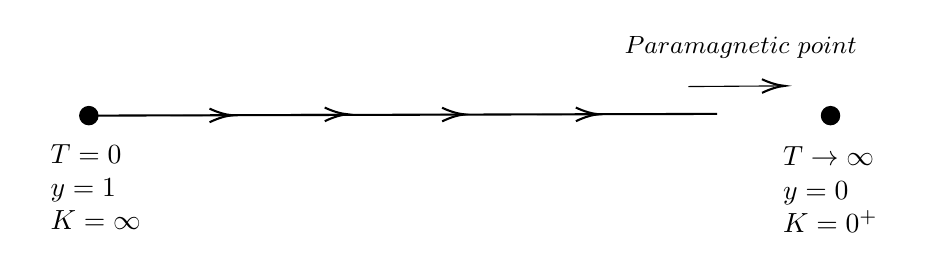
\begin{tikzpicture}[x=0.75pt,y=0.75pt,yscale=-1,xscale=1]
%uncomment if require: \path (0,300); %set diagram left start at 0, and has height of 300

%Straight Lines [id:da20010732884017357] 
\draw [line width=0.75]    (94,109.33) -- (396.75,108.5) ;


%Shape: Circle [id:dp3602066441938294] 
\draw  [fill={rgb, 255:red, 0; green, 0; blue, 0 }  ,fill opacity=1 ] (89.58,109.33) .. controls (89.58,106.89) and (91.56,104.92) .. (94,104.92) .. controls (96.44,104.92) and (98.42,106.89) .. (98.42,109.33) .. controls (98.42,111.77) and (96.44,113.75) .. (94,113.75) .. controls (91.56,113.75) and (89.58,111.77) .. (89.58,109.33) -- cycle ;
%Straight Lines [id:da9616034471654442] 
\draw    (133.33,109.33) -- (161.08,109.18) ;
\draw [shift={(163.08,109.17)}, rotate = 539.6800000000001] [color={rgb, 255:red, 0; green, 0; blue, 0 }  ][line width=0.75]    (10.93,-3.29) .. controls (6.95,-1.4) and (3.31,-0.3) .. (0,0) .. controls (3.31,0.3) and (6.95,1.4) .. (10.93,3.29)   ;

%Straight Lines [id:da10142558241055788] 
\draw    (188.83,108.83) -- (216.58,108.68) ;
\draw [shift={(218.58,108.67)}, rotate = 539.6800000000001] [color={rgb, 255:red, 0; green, 0; blue, 0 }  ][line width=0.75]    (10.93,-3.29) .. controls (6.95,-1.4) and (3.31,-0.3) .. (0,0) .. controls (3.31,0.3) and (6.95,1.4) .. (10.93,3.29)   ;

%Straight Lines [id:da6768117438254937] 
\draw    (245.38,108.92) -- (273.13,108.76) ;
\draw [shift={(275.13,108.75)}, rotate = 539.6800000000001] [color={rgb, 255:red, 0; green, 0; blue, 0 }  ][line width=0.75]    (10.93,-3.29) .. controls (6.95,-1.4) and (3.31,-0.3) .. (0,0) .. controls (3.31,0.3) and (6.95,1.4) .. (10.93,3.29)   ;

%Straight Lines [id:da3997605539627418] 
\draw    (309.83,108.83) -- (337.58,108.68) ;
\draw [shift={(339.58,108.67)}, rotate = 539.6800000000001] [color={rgb, 255:red, 0; green, 0; blue, 0 }  ][line width=0.75]    (10.93,-3.29) .. controls (6.95,-1.4) and (3.31,-0.3) .. (0,0) .. controls (3.31,0.3) and (6.95,1.4) .. (10.93,3.29)   ;

%Straight Lines [id:da6408228695131974] 
\draw    (382.83,95.33) -- (427.25,95.01) ;
\draw [shift={(429.25,95)}, rotate = 539.5899999999999] [color={rgb, 255:red, 0; green, 0; blue, 0 }  ][line width=0.75]    (10.93,-3.29) .. controls (6.95,-1.4) and (3.31,-0.3) .. (0,0) .. controls (3.31,0.3) and (6.95,1.4) .. (10.93,3.29)   ;

%Shape: Circle [id:dp14006527368534316] 
\draw  [fill={rgb, 255:red, 0; green, 0; blue, 0 }  ,fill opacity=1 ] (446.92,109.33) .. controls (446.92,106.89) and (448.89,104.92) .. (451.33,104.92) .. controls (453.77,104.92) and (455.75,106.89) .. (455.75,109.33) .. controls (455.75,111.77) and (453.77,113.75) .. (451.33,113.75) .. controls (448.89,113.75) and (446.92,111.77) .. (446.92,109.33) -- cycle ;

% Text Node
\draw (97.33,145) node    {$ \begin{array}{l}
T=0\\
y=1\\
K=\infty 
\end{array}$};
% Text Node
\draw (451.33,146.33) node    {$ \begin{array}{l}
T\rightarrow \infty \\
y=0\\
K=0^{+}
\end{array}$};
% Text Node
\draw (408,76.67) node  [font=\small]  {$Paramagnetic\ point$};


\end{tikzpicture}

\end{document}
